\documentclass{homeworg}
\usepackage{float}

\title{Theoretical exercise 2}
\author{Håvard Godal}
\begin{document}
\maketitle

\problem
A company producing sea food plans to start using 
an automated classification system to detect possible toxic content 
in blue mussels. The classification will be based on chemical analyses 
of one mussel from each container in a batch of incoming containers of 
newly caught blue mussels, and the concentration x of a specific chemical 
substance in the mussels will be used as feature for classification. 
If this concentration is above a specific threshold value, 
the whole container will be considered poisonous and rejected. 
The company’s gain for each container is NOK 250,-, 
but the company has also issued a guarantee to its customers that if 
they buy a container that shows itself to be poisonous the company 
will compensate costs up to NOK 100000,-.

\bigskip
\textbf{a)} - Let $\omega_1 =$ 'toxic mussels' og $\omega_2 =$ 'non toxic mussels'. Formulate the loss functions $\lambda(\alpha_i|\omega_j),i = 1,2,j = 1,2$, where $\alpha_i$ corresponds to the decision $\omega_i$ (risk will be the same as cost in this setting) when we do not include the possibility of rejecting classifications.
\smallskip

If non toxic mussles are sold and toxic mussles are not sold, the loss is 0.
If a non toxic mussle is not sold, the loss will be 250kr.
If a toxic mussle is sold, the loss will be 100000.

This results in the following loss functions:

\begin{equation}
    \lambda(\alpha_1 | \omega_1) = 0
\end{equation}
\begin{equation}
    \lambda(\alpha_2 | \omega_1) = 100000
\end{equation}
\begin{equation}
    \lambda(\alpha_1 | \omega_2) = 250
\end{equation}
\begin{equation}
    \lambda(\alpha_2 | \omega_2) = 0
\end{equation}

\begin{equation}
    \bm{\lambda}(\alpha_i | \omega_j) = 
    \begin{bmatrix}
        0 & 250 \\
        100000 & 0
    \end{bmatrix}
\end{equation}

\bigskip
\textbf{b)} - Dependent on the value of $x$ we classify as $\omega_1$ or $\omega_2$. Express the conditional loss functions, $R(\alpha_i|x)), i = 1, 2$.
\smallskip
\bigskip

We have that:

\begin{equation}
    p(\bm{x}|\omega_1) \sim N(0.4, 0.0001)
\end{equation}
\begin{equation}
    p(\bm{x}|\omega_2) \sim N(0.2, 0.0001)
\end{equation}
\begin{equation}
    P(\omega_1) = \frac{1}{25}
\end{equation}
\begin{equation}
    P(\omega_2) = \frac{24}{25}
\end{equation}

Furthermore, we can calculate the conditional loss functions like so:

\begin{equation}
    R(\alpha_i|x) = \sum_{j=1}^M \lambda(\alpha_i|\omega_j)*P(\omega_j|x)
\end{equation}

Which results in:
\begin{equation}
    \begin{aligned}
        R(\alpha_1|x) &= \sum_{j=1}^M \lambda(\alpha_1|\omega_j)*P(\omega_j|x)
        \\ &=
        \lambda(\alpha_1|\omega_1)*P(\omega_1|x) + \lambda(\alpha_1|\omega_2)*P(\omega_2|x)
        \\ &=
        0 + 250 * P(\omega_2|x) = 250*\frac{p(x|\omega_2)*P(\omega_2)}{p(x)}
        \\ &=
        250 * P(\omega_2|x) = 250*\frac{p(x|\omega_2)*P(\omega_2)}{P(\omega_1)*p(x|\omega_1) + P(\omega_2)*p(x|\omega_2)}
        \\ &=
        250 * \frac{\frac{1}{0.01*\sqrt{2\pi}}*e^{-\frac{(x-0.2)^2}{0.0002}}*\frac{24}{25}}{\frac{1}{25}*\frac{1}{0.01*\sqrt{2\pi}}*e^{-\frac{(x-0.4)^2}{0.0002}} + \frac{24}{25}*\frac{1}{0.01*\sqrt{2\pi}}*e^{-\frac{(x-0.2)^2}{0.0002}}}
        \\ &=
        \underline{\underline{\frac{6000*e^{-\frac{(x-0.2)^2}{0.0002}}}{e^{-\frac{(x-0.4)^2}{0.0002}} + 24*e^{-\frac{(x-0.2)^2}{0.0002}}}}}
    \end{aligned}
\end{equation}
and:
\begin{equation}
    \begin{aligned}
        R(\alpha_2|x) &= \sum_{j=1}^M \lambda(\alpha_2|\omega_j)*P(\omega_j|x)
        \\ &=
        100000*P(\omega_1|x) + 0 
        \\ &= 
        100000*\frac{p(x|\omega_1)*P(\omega_1)}{p(x)}
        \\ &=
        \underline{\underline{\frac{100000*e^{-\frac{(x-0.4)^2}{0.0002}}}{e^{-\frac{(x-0.4)^2}{0.0002}} + 24*e^{-\frac{(x-0.2)^2}{0.0002}}}}}
    \end{aligned}
\end{equation}


\bigskip
\textbf{c)} - Determine the decision boundary that minimises the overall loss (average cost) upon classification ($R$).
\smallskip

The decision boundary occurs when the conditional loss functions are equal.

\begin{equation}
    \begin{aligned}
        R(\alpha_1|x) &= R(\alpha_2|x) \\
        6000*e^{-\frac{(x-0.2)^2}{0.0002}} &= 100000*e^{-\frac{(x-0.4)^2}{0.0002}} \\
        \ln(6000) -\frac{(x-0.2)^2}{0.0002} &= \ln(100000) -\frac{(x-0.4)^2}{0.0002} \\
        \frac{(x^2 - 0.8x + 0.16) - (x^2 - 0.4x + 0.04)}{0.0002} &= \ln(100000) - \ln(6000) \\
        -2000x + 600 &= \ln(100000) - \ln(6000) \\
        x &= \frac{\ln(100000) - \ln(6000) - 600}{-2000} \\
        x &= x_0 = \underline{\underline{0.2986...}}
    \end{aligned}
\end{equation}


% -------------------------------------------------------------------------------

% According to equation $7.9$ in the textbook, he optimal average risk classifier rule becomes:

% \begin{equation}
%     \text{Assign } \bm{x} \text{ to } \omega_1 (\omega_2) \text{ if}: \lambda_{12} P(\omega_1|\bm{x}) > (<) \lambda_{21} P(\omega_2|\bm{x})
% \end{equation}
% or alternatively:
% \begin{equation}
%     \text{Assign } \bm{x} \text{ to } \omega_1 (\omega_2) \text{ if}: \lambda_{12} P(\omega_1) p(\bm{x}|\omega_1) > (<) \lambda_{21} P(\omega_2) p(\bm{x}|\omega_2)
% \end{equation}

% The decision boundary is found where the two expressions are equal:
% \begin{equation}
%     \lambda_{12} P(\omega_1) p(\bm{x}|\omega_1) = \lambda_{21} P(\omega_2) p(\bm{x}|\omega_2)
% \end{equation}

% Combining equations and solving for x gives:
% \begin{equation}
%     \begin{aligned}
%         \frac{250}{25*0.01\sqrt{2\pi}}e^{-\frac{1}{2} \left(\frac{x-0.4}{0.01}\right)^2} &= 
%         \frac{100000 * 24}{25*0.01\sqrt{2\pi}}e^{-\frac{1}{2} \left(\frac{x-0.2}{0.01}\right)^2}
%         \\
%         250 e^{-\frac{\left(x-0.4\right)^2}{0.0002}} &= 
%         2400000 e^{-\frac{\left(x-0.2\right)^2}{0.0002}}
%         \\
%         \ln(250) - \frac{\left(x-0.4\right)^2}{0.0002} &=
%         \ln(2400000) -\frac{\left(x-0.2\right)^2}{0.0002}
%         \\
%         \frac{(x^2 - 0.4x + 0.04) - (x^2 - 0.8x + 0.16)}{0.0002} &=
%         \ln(2400000) - \ln(250)
%         \\
%         2000x - 600 &=
%         \ln(2400000) - \ln(250)
%         \\
%         x &= \frac{\ln(2400000) - \ln(250) + 600}{2000}
%         \\
%         x &= 0.30458...
%     \end{aligned}
% \end{equation}

% -------------------------------------------------------------------------------

This means that for toxicity concentrations ($x$-values) smaller than $x_0$, the mussels are assumed to be non toxic, and toxic otherwise.


\bigskip
\textbf{d)} - Determine the minimum average cost $R$ upon classification in $NOK$.
\smallskip

The minimum average cost can be found by integrating over the smallest probability density function given $x$.

\begin{equation}
    \begin{aligned}
        R 
        &= \int_{-\infty}^{x_0}R(\alpha_2|x)*p(x)dx + \int_{x_0}^{\infty}R(\alpha_1|x)*p(x)dx \\
        &= \int_{-\infty}^{x_0}\lambda_{12}*P(\omega_1)*p(x|\omega_1)dx + \int_{x_0}^{\infty}\lambda_{21}*P(\omega_2)*p(x|\omega_2)dx \\
        &= \frac{1}{25}100000\int_{-\infty}^{x_0}p(x|\omega_1)dx + \frac{24}{25}250\int_{x_0}^{\infty}p(x|\omega_2)dx \\
        &= 4000 * P(x < x_0|\omega_1) + 240 * P(x > x_0|\omega_2) \\
        &= 4000 * P\left(z < \frac{0.2986-0.4}{0.01}\right) + 240 * \left(1 - P\left(z < \frac{0.2986-0.2}{0.01}\right)\right) \\
        &= 4000 * P(z < -10.14) + 240 * \left(1-P(z < 9.86)\right) \\
        &\approx 4000 * 0 + 240 * (1-1) \\
        &\approx \underline{\underline{0}}
    \end{aligned}
\end{equation}

This means that the probability density functions have almost no overlap, and the chance of misclassification is approximately zero.


\problem
We want to design a pattern recognition system that 
classifies 2-dimensional feature vectors \{$\bm{x}$\} to class 
$\omega_1$, or class $\omega_2$.

It is known that the distribution between the two classes are 
1/2 and 1/2 respectively for class $\omega_1$ and class $\omega_2$. 
Furthermore the feature vectors of the two classes are normally 
distributed around $\mu_1 = (3 \: 3)^T$ with covariance matrix
\begin{equation}
    \bm{\Sigma_1} =
    \begin{bmatrix}
        1/2 & 0 \\
        0 & 2
    \end{bmatrix}
\end{equation}
for class $\omega_1$, og around $\mu_2 = (3 - 2)^T$ with covariance matrix
\begin{equation}
    \bm{\Sigma_2} = 
    \begin{bmatrix}
        2 & 0 \\
        0 & 2
    \end{bmatrix}
\end{equation}
for class $\omega_2$

The eigenvalue and eigenvector matrices $\bm{\Lambda}_i$ and $\bm{\Phi}_i$, 
$i = 1, 2$ for the convariance matrices are
\begin{equation}
    \bm{\Lambda_1} =
    \begin{bmatrix}
        1/2 & 0 \\
        0 & 2
    \end{bmatrix}
\end{equation}
and
\begin{equation}
    \bm{\Phi_1} =
    \begin{bmatrix}
        1 & 0 \\
        0 & 1
    \end{bmatrix}
\end{equation}
for class $\omega_1$, and
\begin{equation}
    \bm{\Lambda_2} =
    \begin{bmatrix}
        2 & 0 \\
        0 & 2
    \end{bmatrix}
\end{equation}
and
\begin{equation}
    \bm{\Phi_2} =
    \begin{bmatrix}
        1 & 0 \\
        0 & 1
    \end{bmatrix}
\end{equation}
for class $\omega_2$ respectively.

\bigskip
\textbf{a)} - Sketch the contour lines for the class specific probability density functions for the two classes in the same diagram.
\smallskip

\begin{figure}[H]
    \centering
    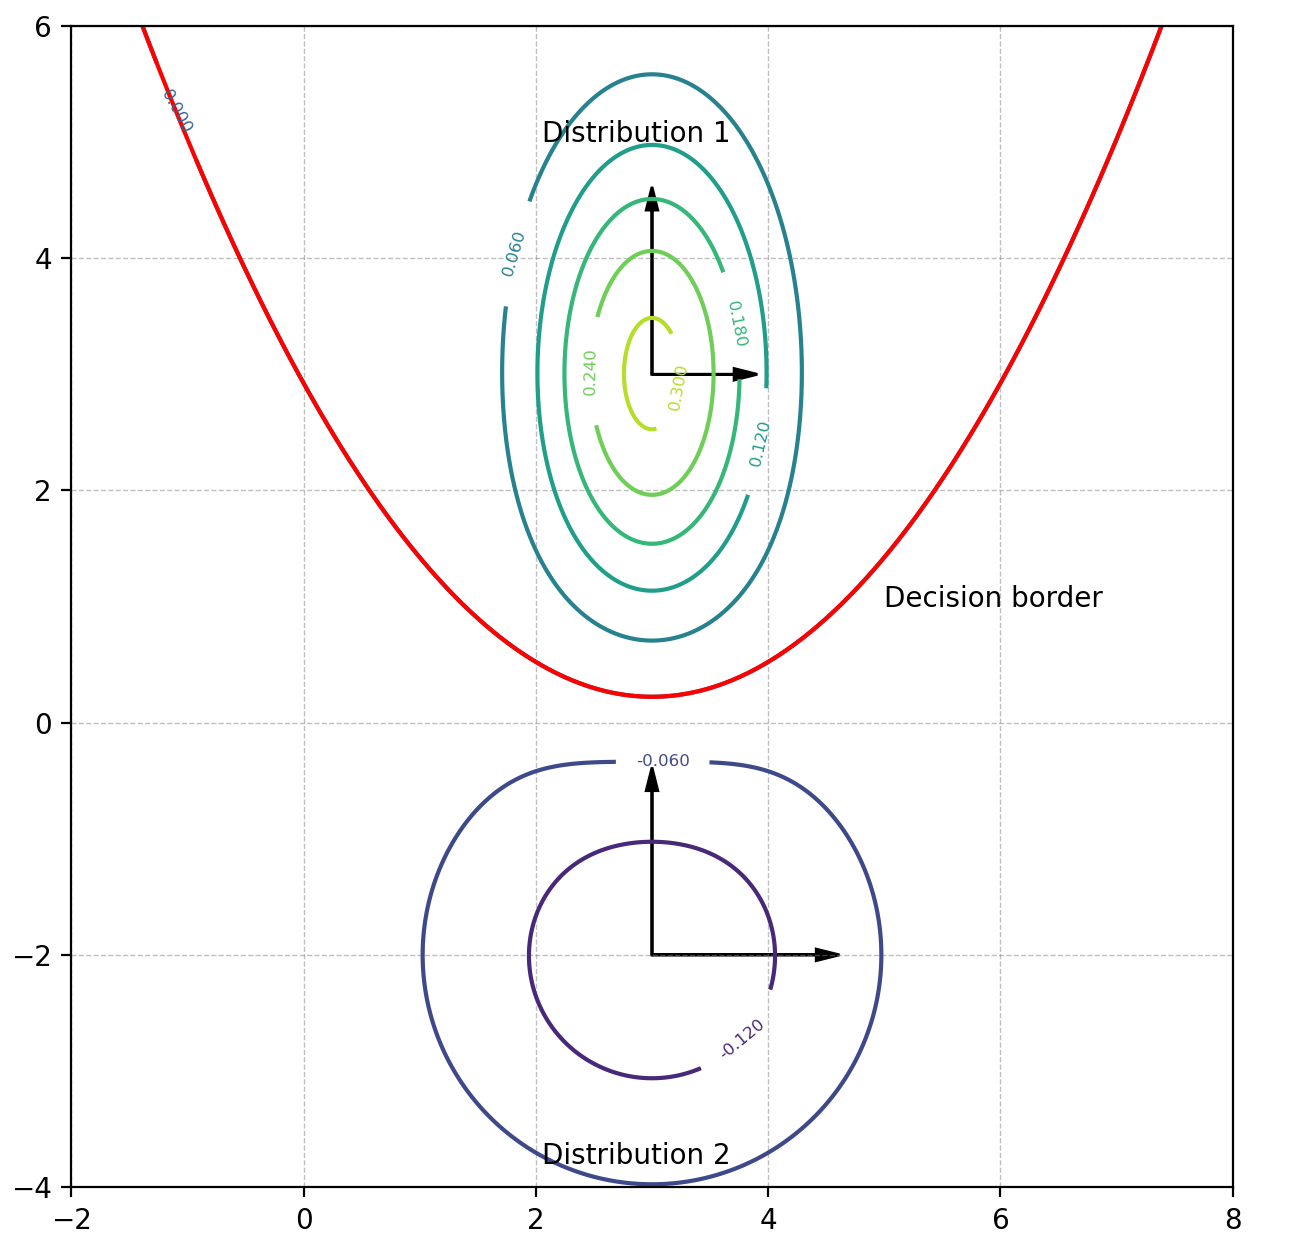
\includegraphics[scale=0.7]{Figure2.png}
    \caption{Contour lines for the class conditional density functions}
\end{figure}


\bigskip
\textbf{b)} - Formulate Bayes decision rule for this problem. Determine the decision boundary and decision regions in the same diagram as in a).
\smallskip

Bayes decision rule is as follows:
\begin{equation}
    \text{Decide }
    \left\{\begin{matrix*}[l]
        \omega_1& \text{if } P(\omega_1|\bm{x}) > P(\omega_2|\bm{x})\\ 
        \omega_2& \text{otherwise} 
       \end{matrix*}\right.
\end{equation}

And from the exercise notes:
\begin{equation}
    g_i(\bm{x}) = \bm{x}^T\bm{\Theta}_i\bm{x}+\bm{\theta}_i^T\bm{x}+\theta_{i0}
\end{equation}
where:
\begin{equation}
    \begin{aligned}
        \bm{\Theta}_i &= -\frac{1}{2}\Sigma_i^{-1} \\
        \bm{\theta}_i &= \Sigma_i^{-1}\bm{\mu}_i \\
        \theta_{i0} &= -\frac{1}{2}\mu_i^T\Sigma_i^{-1}\mu_i-\frac{1}{2}\ln\abs{\Sigma_i}+\ln(P(\omega_i))
    \end{aligned}
\end{equation}

Solving for $g_1(\bm{x})$:

\begin{equation}
    \begin{aligned}
        \bm{\Theta}_1 &= -\frac{1}{2}
        \begin{bmatrix}
            2 & 0 \\
            0 & 1/2
        \end{bmatrix}
        \\ &=
        \begin{bmatrix}
            -1 & 0 \\
            0 & -1/4
        \end{bmatrix}
    \end{aligned}
\end{equation}

\begin{equation}
    \begin{aligned}
        \bm{\theta}_1 &=
        \begin{bmatrix}
            2 & 0 \\
            0 & 1/2
        \end{bmatrix}
        \begin{bmatrix}
            3 \\ 3
        \end{bmatrix}
        \\ &=
        \begin{bmatrix}
            6 \\
            3/2
        \end{bmatrix}
    \end{aligned}
\end{equation}

\begin{equation}
    \begin{aligned}
        {\theta}_{10} &=
        -\frac{1}{2}
        \begin{bmatrix}
            3 & 3
        \end{bmatrix}
        \begin{bmatrix}
            2 & 0 \\ 0 & 1/2
        \end{bmatrix}
        \begin{bmatrix}
            3 \\ 3
        \end{bmatrix}
        -\frac{1}{2}\ln(1/2*2+0*0)+\ln(1/2)
        \\ &= -11.943
    \end{aligned}
\end{equation}

\begin{equation}
    \begin{aligned}
        g_1(\bm{x}) &=
        \begin{bmatrix}
            x_1 & x_2
        \end{bmatrix}
        \begin{bmatrix}
            -1 & 0 \\
            0 & -1/4
        \end{bmatrix}
        \begin{bmatrix}
            x_1 \\ x_2
        \end{bmatrix} + 
        \begin{bmatrix}
            6 & 3/2
        \end{bmatrix}
        \begin{bmatrix}
            x_1 \\ x_2
        \end{bmatrix} - 11.943
        \\ &=
        -x_1^2-\frac{1}{4}x_2^2+6x_1+\frac{3}{2}x_2-11.943
    \end{aligned}
\end{equation}


Solving for $g_2(\bm{x})$:

\begin{equation}
    \begin{aligned}
        \bm{\Theta}_2 &= -\frac{1}{2}
        \begin{bmatrix}
            1/2 & 0 \\
            0 & 1/2
        \end{bmatrix}
        \\ &=
        \begin{bmatrix}
            -1/4 & 0 \\
            0 & -1/4
        \end{bmatrix}
    \end{aligned}
\end{equation}

\begin{equation}
    \begin{aligned}
        \bm{\theta}_2 &=
        \begin{bmatrix}
            1/2 & 0 \\
            0 & 1/2
        \end{bmatrix}
        \begin{bmatrix}
            3 \\ 2-
        \end{bmatrix}
        \\ &=
        \begin{bmatrix}
            3/2 \\
            -1
        \end{bmatrix}
    \end{aligned}
\end{equation}

\begin{equation}
    \begin{aligned}
        {\theta}_{20} &=
        -\frac{1}{2}
        \begin{bmatrix}
            3 & -2
        \end{bmatrix}
        \begin{bmatrix}
            1/2 & 0 \\ 0 & 1/2
        \end{bmatrix}
        \begin{bmatrix}
            3 \\ -2
        \end{bmatrix}
        -\frac{1}{2}\ln(2*2+0*0)+\ln(1/2)
        \\ &= -4.636
    \end{aligned}
\end{equation}

\begin{equation}
    \begin{aligned}
        g_2(\bm{x}) &=
        \begin{bmatrix}
            x_1 & x_2
        \end{bmatrix}
        \begin{bmatrix}
            -1/4 & 0 \\
            0 & -1/4
        \end{bmatrix}
        \begin{bmatrix}
            x_1 \\ x_2
        \end{bmatrix} + 
        \begin{bmatrix}
            -2 & 3
        \end{bmatrix}
        \begin{bmatrix}
            x_1 \\ x_2
        \end{bmatrix} -4.636
        \\ &=
        -\frac{1}{4}x_1^2-\frac{1}{4}x_2^2+\frac{3}{2}x_1-x_2-4.636
    \end{aligned}
\end{equation}

The decision border occurs when $g_1(\bm{x}) = g_2(\bm{x})$
\begin{equation}
    \begin{aligned}
        g_1(\bm{x}) &= g_2(\bm{x}) \\
        -x_1^2+6x_1-\frac{1}{4}x_2^2+\frac{3}{2}x_2-11.943 &= -\frac{1}{4}x_1^2-\frac{1}{4}x_2^2+\frac{3}{2}x_1-x_2-4.636
        \\
        -\frac{3}{4}x_1^2
        +\frac{9}{2}x_1
        +\frac{5}{2}x_2
        -7.307
        &= 0 \\
        x_2
        &=\frac{3}{10}x_1^2-\frac{9}{5}x_1+2.923
    \end{aligned}
\end{equation}




\problem
Show that with
\begin{equation}
    g_i(\bm{x}) = - \frac{\norm{\bm{x} - \bm{\mu}_i}^2}{2\sigma^2} + \ln P(\omega_i)
\end{equation}
as a starting point where $i = 1, 2$, we can reach an expression defining the decision border between the two classes:
\begin{equation}
    \bm{\theta}^T(\bm{x}-\bm{x_0}) = 0
\end{equation}
where
\begin{equation}
    \bm{\theta} = \bm{\mu}_i - \bm{\mu}_j 
\end{equation}
and
\begin{equation}
    \bm{x_0} = \frac{1}{2}(\bm{\mu}_i + \bm{\mu}_j) - \frac{\sigma^2}{\norm{\bm{\mu}_i + \bm{\mu}_j}^2} \ln \frac{P(\omega_i)}{P(\omega_j)}(\bm{\mu}_i + \bm{\mu}_j)
\end{equation}

From the lecture notes, the following calculations can be done with $g_i(\bm{x})$:
\begin{equation}
    \begin{aligned}
        g_i(\bm{x}) &= -\frac{1}{2\sigma^2} \left(\bm{x}- \bm{\mu}_i\right)^T\left(\bm{x}- \bm{\mu}_i\right) + \ln(P(\omega_i))
        \\
        &= -\frac{1}{2\sigma^2} \left[\bm{x}^T\bm{x}-2\bm{\mu}_i^T\bm{x}+\bm{\mu}_i^T\bm{\mu}_i\right] + \ln(P(\omega_i))
        \\
        & \text{Removing the class independent terms}
        \\
        &= -\frac{1}{2\sigma^2} \left[-2\bm{\mu}_i^T\bm{x}+\bm{\mu}_i^T\bm{\mu}_i\right] + \ln(P(\omega_i))
    \end{aligned}
\end{equation}

Setting $g_i(\bm{x}) = g_j(\bm{x})$
\begin{equation}
    \begin{aligned}
        -\frac{1}{2\sigma^2} \left[-2\bm{\mu}_i^T\bm{x}+\bm{\mu}_i^T\bm{\mu}_i\right] + \ln(P(\omega_i)) =
        -\frac{1}{2\sigma^2} \left[-2\bm{\mu}_j^T\bm{x}+\bm{\mu}_j^T\bm{\mu}_j\right] + \ln(P(\omega_j))
        \\
        -\frac{1}{2\sigma^2} \left[-2\bm{\mu}_i^T\bm{x}+\bm{\mu}_i^T\bm{\mu}_i\right]
        +\frac{1}{2\sigma^2} \left[-2\bm{\mu}_j^T\bm{x}+\bm{\mu}_j^T\bm{\mu}_j\right] + \ln(P(\omega_i)) - \ln(P(\omega_j)) =0
        \\
        -\frac{1}{2} \left[-2\bm{\mu}_i^T\bm{x}+\bm{\mu}_i^T\bm{\mu}_i\right]
        +\frac{1}{2} \left[-2\bm{\mu}_j^T\bm{x}+\bm{\mu}_j^T\bm{\mu}_j\right] + \sigma^2 \ln\left(\frac{P(\omega_i)}{P(\omega_j)}\right)=0
        \\
        \left(\bm{\mu}_i-\bm{\mu}_j\right)^T\bm{x}
        - \frac{1}{2} \bm{\mu}_i^T\bm{\mu}_i
        + \frac{1}{2} \bm{\mu}_j^T\bm{\mu}_j
        + \sigma^2 \ln\left(\frac{P(\omega_i)}{P(\omega_j)}\right)=0
        \\
        \text{Expanding the expression with } \frac{1}{2}\left(\bm{\mu}_i^T\bm{\mu}_j - \bm{\mu}_j^T\bm{\mu}_j\right) (\text{which equals }0)
        \\
        \left(\bm{\mu}_i-\bm{\mu}_j\right)^T\bm{x}
        - \frac{1}{2} \left(\bm{\mu}_i - \bm{\mu}_j\right)^T\left(\bm{\mu}_i + \bm{\mu}_j\right)
        + \sigma^2 \ln\left(\frac{P(\omega_i)}{P(\omega_j)}\right)=0
        \\
        \text{To write the expression in the desired form, the last term is extended.}
        \\
        \left(\bm{\mu}_i-\bm{\mu}_j\right)^T\bm{x}
        - \frac{1}{2} \left(\bm{\mu}_i - \bm{\mu}_j\right)^T\left(\bm{\mu}_i + \bm{\mu}_j\right)
        + \sigma^2 \ln\left(\frac{P(\omega_i)}{P(\omega_j)}\right)\frac{\left(\bm{\mu}_i - \bm{\mu}_j\right)^T\left(\bm{\mu}_i - \bm{\mu}_j\right)}{\left(\bm{\mu}_i - \bm{\mu}_j\right)^T\left(\bm{\mu}_i - \bm{\mu}_j\right)}=0 \\
        \text{Rewriting the denominator and moving equal terms outside the parentheses.} \\
        \left(\bm{\mu}_i - \bm{\mu}_j\right)^T\left[\bm{x} - \left(\frac{1}{2}\left(\bm{\mu}_i + \bm{\mu}_j\right)-\frac{\sigma^2}{\norm{\bm{\mu}_i-\bm{\mu}_j}^2}\ln\frac{P(\omega_i)}{P(\omega_j)}\left(\bm{\mu}_i-\bm{\mu}_j\right)\right)\right]&=0
        \\
        \text{Which equals to:}
        \\
        \bm{\theta}^T(\bm{x}-\bm{x_0}) &= 0
    \end{aligned}
\end{equation}


\end{document}
